\documentclass{standalone}
\usepackage{tikz}
\usetikzlibrary{patterns, positioning}
\usepackage[sfdefault]{ClearSans} %% option 'sfdefault' activates Clear Sans as the default text font
\usepackage[T1]{fontenc}

\begin{document}
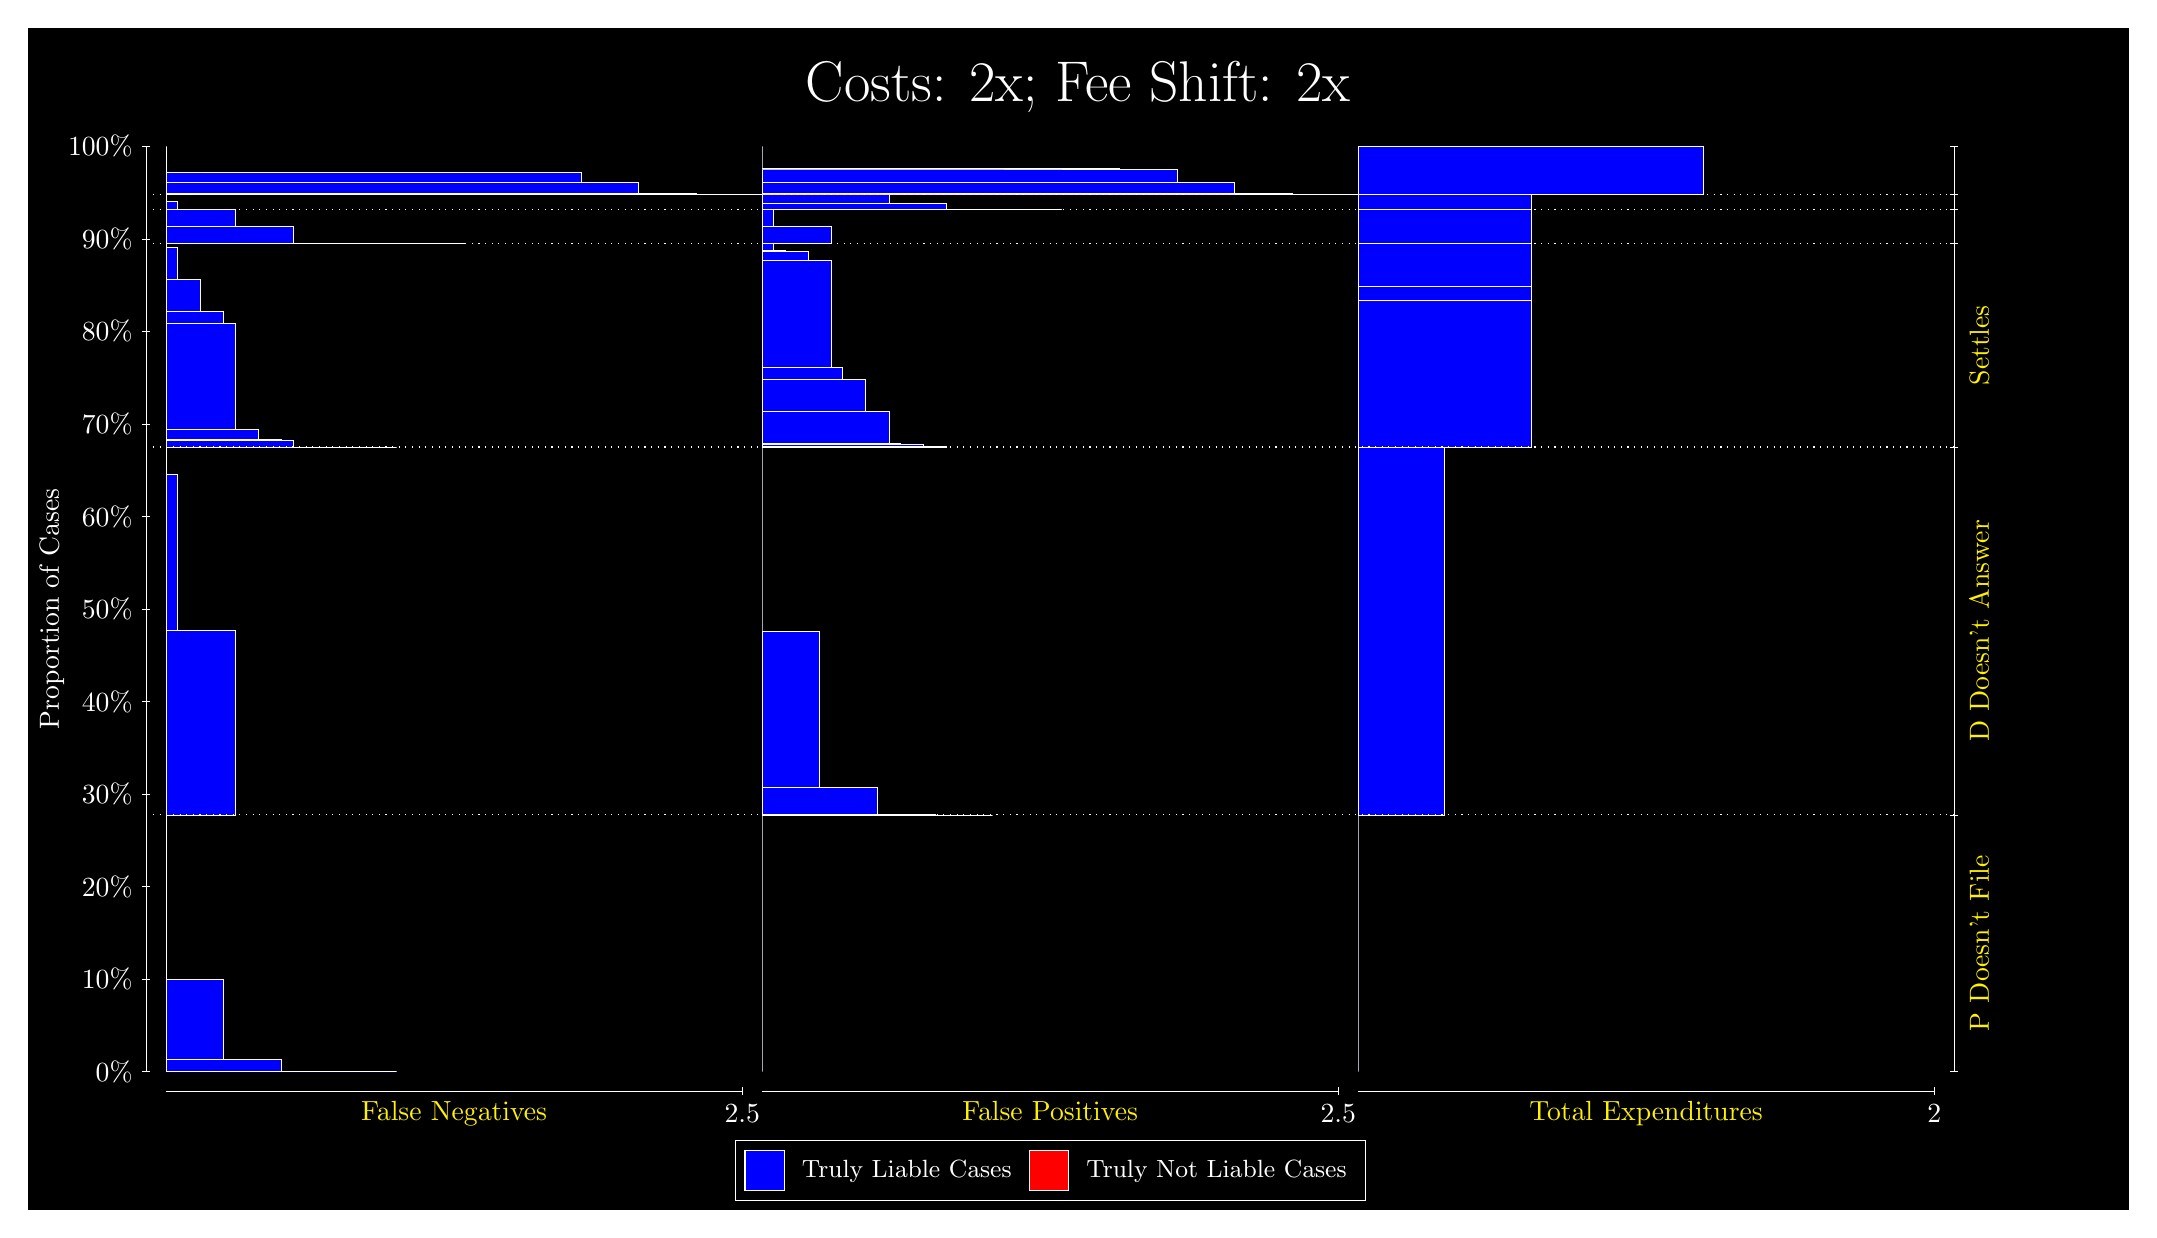
\begin{tikzpicture}
\draw[fill=black] (0,0) rectangle (26.667,15);
\draw[text=white] (0,13.5) rectangle (26.667,15) node[midway] {\huge Costs: 2x; Fee Shift: 2x};
\draw[white, very thin] (1.5,1.75) -- (1.5,13.5);
\node[rotate=90, text=white, anchor=center] at (0.3, 7.625) {Proportion of Cases};
\draw[white, very thin] (1.45,1.75) -- (1.55,1.75);
\node[text=white, anchor=east] at (1.45, 1.75) {0\%};
\draw[white, very thin] (1.45,2.925) -- (1.55,2.925);
\node[text=white, anchor=east] at (1.45, 2.925) {10\%};
\draw[white, very thin] (1.45,4.1) -- (1.55,4.1);
\node[text=white, anchor=east] at (1.45, 4.1) {20\%};
\draw[white, very thin] (1.45,5.275) -- (1.55,5.275);
\node[text=white, anchor=east] at (1.45, 5.275) {30\%};
\draw[white, very thin] (1.45,6.45) -- (1.55,6.45);
\node[text=white, anchor=east] at (1.45, 6.45) {40\%};
\draw[white, very thin] (1.45,7.625) -- (1.55,7.625);
\node[text=white, anchor=east] at (1.45, 7.625) {50\%};
\draw[white, very thin] (1.45,8.8) -- (1.55,8.8);
\node[text=white, anchor=east] at (1.45, 8.8) {60\%};
\draw[white, very thin] (1.45,9.975) -- (1.55,9.975);
\node[text=white, anchor=east] at (1.45, 9.975) {70\%};
\draw[white, very thin] (1.45,11.15) -- (1.55,11.15);
\node[text=white, anchor=east] at (1.45, 11.15) {80\%};
\draw[white, very thin] (1.45,12.325) -- (1.55,12.325);
\node[text=white, anchor=east] at (1.45, 12.325) {90\%};
\draw[white, very thin] (1.45,13.5) -- (1.55,13.5);
\node[text=white, anchor=east] at (1.45, 13.5) {100\%};

\draw[white, very thin] (24.457,1.75) -- (24.457,13.5);
\draw[white, very thin] (24.407,1.75) -- (24.507,1.75);
\node[anchor=west] at (24.407, 1.75) {};
\draw[white, very thin] (24.407,5.0096) -- (24.507,5.0096);
\node[anchor=west] at (24.407, 5.0096) {};
\draw[white, very thin] (24.407,9.6818) -- (24.507,9.6818);
\node[anchor=west] at (24.407, 9.6818) {};
\draw[white, very thin] (24.407,12.266) -- (24.507,12.266);
\node[anchor=west] at (24.407, 12.266) {};
\draw[white, very thin] (24.407,12.699) -- (24.507,12.699);
\node[anchor=west] at (24.407, 12.699) {};
\draw[white, very thin] (24.407,12.889) -- (24.507,12.889);
\node[anchor=west] at (24.407, 12.889) {};
\draw[white, very thin] (24.407,13.5) -- (24.507,13.5);
\node[anchor=west] at (24.407, 13.5) {};

\draw[white, very thin, fill=blue] (1.75,1.75) rectangle (4.6775,1.75);
\draw[white, very thin, fill=blue] (1.75,1.75) rectangle (3.9457,1.7513);
\draw[white, very thin, fill=blue] (1.75,1.7513) rectangle (3.2138,1.9042);
\draw[white, very thin, fill=blue] (1.75,1.9042) rectangle (2.4819,2.9249);
\draw[white, very thin, fill=red] (1.75,2.9249) rectangle (1.75,2.9249);
\draw[white, very thin, fill=blue] (1.75,2.9249) rectangle (1.75,5.0096);
\draw[white, very thin, fill=blue] (1.75,5.0096) rectangle (2.6283,7.3558);
\draw[white, very thin, fill=blue] (1.75,7.3558) rectangle (1.8964,9.3314);
\draw[white, very thin, fill=red] (1.75,9.3314) rectangle (1.75,9.3314);
\draw[white, very thin, fill=blue] (1.75,9.3314) rectangle (1.75,9.6818);
\draw[white, very thin, fill=blue] (1.75,9.6818) rectangle (4.6775,9.6818);
\draw[white, very thin, fill=blue] (1.75,9.6818) rectangle (4.3848,9.6818);
\draw[white, very thin, fill=blue] (1.75,9.6818) rectangle (4.092,9.6819);
\draw[white, very thin, fill=blue] (1.75,9.6819) rectangle (3.9457,9.6819);
\draw[white, very thin, fill=blue] (1.75,9.6819) rectangle (3.6529,9.6821);
\draw[white, very thin, fill=blue] (1.75,9.6821) rectangle (3.3602,9.7729);
\draw[white, very thin, fill=blue] (1.75,9.7729) rectangle (3.2138,9.781);
\draw[white, very thin, fill=blue] (1.75,9.781) rectangle (2.921,9.9005);
\draw[white, very thin, fill=blue] (1.75,9.9005) rectangle (2.6283,11.252);
\draw[white, very thin, fill=blue] (1.75,11.252) rectangle (2.4819,11.409);
\draw[white, very thin, fill=blue] (1.75,11.409) rectangle (2.1891,11.811);
\draw[white, very thin, fill=blue] (1.75,11.811) rectangle (1.8964,12.217);
\draw[white, very thin, fill=red] (1.75,12.217) rectangle (1.75,12.217);
\draw[white, very thin, fill=blue] (1.75,12.217) rectangle (1.75,12.266);
\draw[white, very thin, fill=blue] (1.75,12.266) rectangle (5.5558,12.266);
\draw[white, very thin, fill=blue] (1.75,12.266) rectangle (4.8239,12.266);
\draw[white, very thin, fill=blue] (1.75,12.266) rectangle (4.092,12.27);
\draw[white, very thin, fill=blue] (1.75,12.27) rectangle (3.3602,12.486);
\draw[white, very thin, fill=blue] (1.75,12.486) rectangle (2.6283,12.699);
\draw[white, very thin, fill=red] (1.75,12.699) rectangle (1.75,12.699);
\draw[white, very thin, fill=blue] (1.75,12.699) rectangle (2.6283,12.7);
\draw[white, very thin, fill=blue] (1.75,12.7) rectangle (1.8964,12.805);
\draw[white, very thin, fill=red] (1.75,12.805) rectangle (1.75,12.805);
\draw[white, very thin, fill=blue] (1.75,12.805) rectangle (1.75,12.889);
\draw[white, very thin, fill=blue] (1.75,12.889) rectangle (9.9471,12.889);
\draw[white, very thin, fill=blue] (1.75,12.889) rectangle (9.2152,12.889);
\draw[white, very thin, fill=blue] (1.75,12.889) rectangle (8.4834,12.899);
\draw[white, very thin, fill=blue] (1.75,12.899) rectangle (7.7515,13.039);
\draw[white, very thin, fill=blue] (1.75,13.039) rectangle (7.0196,13.173);
\draw[white, very thin, fill=blue] (1.75,13.173) rectangle (6.2877,13.173);
\draw[white, very thin, fill=blue] (1.75,13.173) rectangle (5.5558,13.173);
\draw[white, very thin, fill=blue] (1.75,13.173) rectangle (2.1891,13.173);
\draw[white, very thin, fill=red] (1.75,13.173) rectangle (1.75,13.173);
\draw[white, very thin, fill=blue] (1.75,13.173) rectangle (1.75,13.5);
\draw[white, very thin, fill=red] (9.3189,1.75) rectangle (9.3189,1.75);
\draw[white, very thin, fill=blue] (9.3189,1.75) rectangle (9.3189,5.0096);
\draw[white, very thin, fill=red] (9.3189,5.0096) rectangle (12.246,5.0096);
\draw[white, very thin, fill=blue] (9.3189,5.0096) rectangle (12.246,5.0096);
\draw[white, very thin, fill=blue] (9.3189,5.0096) rectangle (11.515,5.0114);
\draw[white, very thin, fill=blue] (9.3189,5.0114) rectangle (10.783,5.36);
\draw[white, very thin, fill=blue] (9.3189,5.36) rectangle (10.051,7.3356);
\draw[white, very thin, fill=blue] (9.3189,7.3356) rectangle (9.3189,9.6818);
\draw[white, very thin, fill=red] (9.3189,9.6818) rectangle (11.661,9.6818);
\draw[white, very thin, fill=blue] (9.3189,9.6818) rectangle (11.661,9.6924);
\draw[white, very thin, fill=red] (9.3189,9.6924) rectangle (11.368,9.6924);
\draw[white, very thin, fill=blue] (9.3189,9.6924) rectangle (11.368,9.7149);
\draw[white, very thin, fill=red] (9.3189,9.7149) rectangle (11.075,9.7149);
\draw[white, very thin, fill=blue] (9.3189,9.7149) rectangle (11.075,9.7313);
\draw[white, very thin, fill=blue] (9.3189,9.7313) rectangle (10.929,10.137);
\draw[white, very thin, fill=blue] (9.3189,10.137) rectangle (10.636,10.539);
\draw[white, very thin, fill=blue] (9.3189,10.539) rectangle (10.344,10.696);
\draw[white, very thin, fill=blue] (9.3189,10.696) rectangle (10.197,12.048);
\draw[white, very thin, fill=blue] (9.3189,12.048) rectangle (9.9044,12.167);
\draw[white, very thin, fill=blue] (9.3189,12.167) rectangle (9.6116,12.175);
\draw[white, very thin, fill=blue] (9.3189,12.175) rectangle (9.4652,12.266);
\draw[white, very thin, fill=blue] (9.3189,12.266) rectangle (9.3189,12.266);
\draw[white, very thin, fill=red] (9.3189,12.266) rectangle (10.197,12.266);
\draw[white, very thin, fill=blue] (9.3189,12.266) rectangle (10.197,12.479);
\draw[white, very thin, fill=blue] (9.3189,12.479) rectangle (9.4652,12.695);
\draw[white, very thin, fill=blue] (9.3189,12.695) rectangle (9.3189,12.699);
\draw[white, very thin, fill=red] (9.3189,12.699) rectangle (13.125,12.699);
\draw[white, very thin, fill=blue] (9.3189,12.699) rectangle (13.125,12.699);
\draw[white, very thin, fill=blue] (9.3189,12.699) rectangle (12.393,12.699);
\draw[white, very thin, fill=blue] (9.3189,12.699) rectangle (11.661,12.782);
\draw[white, very thin, fill=blue] (9.3189,12.782) rectangle (10.929,12.887);
\draw[white, very thin, fill=blue] (9.3189,12.887) rectangle (10.197,12.889);
\draw[white, very thin, fill=red] (9.3189,12.889) rectangle (17.516,12.889);
\draw[white, very thin, fill=blue] (9.3189,12.889) rectangle (17.516,12.889);
\draw[white, very thin, fill=red] (9.3189,12.889) rectangle (16.784,12.889);
\draw[white, very thin, fill=blue] (9.3189,12.889) rectangle (16.784,12.889);
\draw[white, very thin, fill=red] (9.3189,12.889) rectangle (16.052,12.889);
\draw[white, very thin, fill=blue] (9.3189,12.889) rectangle (16.052,12.899);
\draw[white, very thin, fill=red] (9.3189,12.899) rectangle (15.32,12.899);
\draw[white, very thin, fill=blue] (9.3189,12.899) rectangle (15.32,13.04);
\draw[white, very thin, fill=blue] (9.3189,13.04) rectangle (14.588,13.214);
\draw[white, very thin, fill=blue] (9.3189,13.214) rectangle (13.857,13.215);
\draw[white, very thin, fill=blue] (9.3189,13.215) rectangle (13.125,13.215);
\draw[white, very thin, fill=blue] (9.3189,13.215) rectangle (12.393,13.215);
\draw[white, very thin, fill=red] (9.3189,13.215) rectangle (9.3189,13.215);
\draw[white, very thin, fill=blue] (9.3189,13.215) rectangle (9.3189,13.5);
\draw[white, very thin, fill=red] (16.888,1.75) rectangle (16.888,1.75);
\draw[white, very thin, fill=blue] (16.888,1.75) rectangle (16.888,5.0096);
\draw[white, very thin, fill=red] (16.888,5.0096) rectangle (17.986,5.0096);
\draw[white, very thin, fill=blue] (16.888,5.0096) rectangle (17.986,9.6818);
\draw[white, very thin, fill=red] (16.888,9.6818) rectangle (19.083,9.6818);
\draw[white, very thin, fill=blue] (16.888,9.6818) rectangle (19.083,11.541);
\draw[white, very thin, fill=red] (16.888,11.541) rectangle (19.083,11.541);
\draw[white, very thin, fill=blue] (16.888,11.541) rectangle (19.083,11.722);
\draw[white, very thin, fill=red] (16.888,11.722) rectangle (19.083,11.722);
\draw[white, very thin, fill=blue] (16.888,11.722) rectangle (19.083,12.266);
\draw[white, very thin, fill=red] (16.888,12.266) rectangle (19.083,12.266);
\draw[white, very thin, fill=blue] (16.888,12.266) rectangle (19.083,12.699);
\draw[white, very thin, fill=red] (16.888,12.699) rectangle (19.083,12.699);
\draw[white, very thin, fill=blue] (16.888,12.699) rectangle (19.083,12.889);
\draw[white, very thin, fill=red] (16.888,12.889) rectangle (21.279,12.889);
\draw[white, very thin, fill=blue] (16.888,12.889) rectangle (21.279,13.5);
\draw[white, dotted] (1.5,5.0096) -- (24.457,5.0096);
\draw[white, dotted] (1.5,9.6818) -- (24.457,9.6818);
\draw[white, dotted] (1.5,12.266) -- (24.457,12.266);
\draw[white, dotted] (1.5,12.699) -- (24.457,12.699);
\draw[white, dotted] (1.5,12.889) -- (24.457,12.889);
\draw[white, very thin] (1.75,1.5) -- (9.0689,1.5);
\node[text=yellow, anchor=north] at (5.4094, 1.5) {False Negatives};
\draw[white, very thin] (9.0689,1.45) -- (9.0689,1.55);
\node[text=white, anchor=north] at (9.0689, 1.45) {2.5};

\draw[white, very thin] (9.3189,1.5) -- (16.638,1.5);
\node[text=yellow, anchor=north] at (12.978, 1.5) {False Positives};
\draw[white, very thin] (16.638,1.45) -- (16.638,1.55);
\node[text=white, anchor=north] at (16.638, 1.45) {2.5};

\draw[white, very thin] (16.888,1.5) -- (24.207,1.5);
\node[text=yellow, anchor=north] at (20.547, 1.5) {Total Expenditures};
\draw[white, very thin] (24.207,1.45) -- (24.207,1.55);
\node[text=white, anchor=north] at (24.207, 1.45) {2};

\node[text=yellow, centered, rotate=90] at (24.777, 3.3798) {P Doesn't File};
\node[text=yellow, centered, rotate=90] at (24.777, 7.3457) {D Doesn't Answer};
\node[text=yellow, centered, rotate=90] at (24.777, 10.974) {Settles};




\draw (12.978300999999998,1.5) node[draw=none] (baseCoordinate) {};
\begin{scope}[align=center]
        \matrix[scale=0.5, draw=white, below=0.5cm of baseCoordinate, nodes={draw}, column sep=0.1cm]{
            \node[rectangle, draw, minimum width=0.5cm, minimum height=0.5cm, fill=blue] {}; &
            \node[draw=none, font=\small, text=white] (B) {Truly Liable Cases}; &
            \node[rectangle, draw, minimum width=0.5cm, minimum height=0.5cm, fill=red] {}; &
            \node[draw=none, font=\small, text=white] (B) {Truly Not Liable Cases}; \\
            };
\end{scope}

\end{tikzpicture}
\end{document}